% Status: DRAFT. Measurement paper: what reference matching measures.
% Assembled from paper_latex/main.tex (authoritative numbers) with narrative framing from
% papers/B-reference-matching/seed-paper1.md. Judge-certification and selection-pressure
% material deliberately excluded (separate papers).
% Anchor-set numbers retrofitted to papers/analysis/canonical_validity.md (canonical analysis).
% !TEX root = main.tex
\documentclass[11pt]{article}
\usepackage[margin=1in]{geometry}
\usepackage{amsmath,amssymb}
\usepackage{graphicx}
\usepackage{booktabs}
\usepackage{multirow}
\usepackage{xcolor}
\usepackage[colorlinks=true,linkcolor=blue,citecolor=blue,urlcolor=blue]{hyperref}
\usepackage{caption}
\captionsetup{font=small,labelfont=bf}

\newcommand{\tfa}{\textsc{TFA}}
\newcommand{\judgetbd}{$+0.89$}

\title{What Does Matching a Reference Actually Measure?\\ \large Comparison metrics measure the reference; verification signals grade the solution}
\author{Anonymous Authors}
\date{Draft, August 22, 2026}

\begin{document}
\maketitle

\begin{abstract}
% 1 problem motivation
Many benchmarks ship a gold reference solution, so the cheapest way to evaluate a model's reasoning is to score a solution by how much it resembles that reference.
% 2 the question
We ask what reference matching actually measures, across seventeen models from seven families on eight math and code benchmarks, anchored to blind human grades of reasoning quality and to executed tests.
% 3 finding 1: ranking boundary
Matching can rank models, but only when the reference is worth predicting.
Replacing each worked reference with its answer line collapses the ranking signal on the same items (Spearman $+0.35 \to +0.02$), and the boundary runs from $+0.86$ on olympiad math into reversal on saturated data.
% 4 finding 2: grading null + mechanism
No form of matching can grade an individual solution.
Five metrics spanning the space, from teacher-forced accuracy to sentence embeddings, land in $[-0.33, +0.14]$ against human soundness grades and at $0.00$ against executed tests on 492 code solutions.
The reason is mechanistic: $83$--$92\%$ of per-solution variance beyond model level is reference-specific nuisance, and pooled across 6{,}000 model--item pairs, teacher-forced accuracy is $80\%$ reference perplexity.
Every targeted repair we or our reviewers proposed failed exactly as pre-registered predictions said it would.
% 5 finding 3: what grades
What does grade is verification.
Executed tests are a free oracle where they exist, and a prefix-repair curve, which truncates a solution and asks whether a fixed completer still reaches the right answer, correlates at $+0.79$ with human soundness with no LLM judge involved, at the human inter-rater ceiling.
% 6 implications
Two rules follow: use a reference as an endpoint for a verifier, never as a similarity target, and for leaderboards, report reference entropy alongside accuracy, because matching is legitimate exactly when references are worth predicting.
\end{abstract}

\section{Introduction}
\label{sec:intro}

% P1: problem motivation
Most benchmarks that matter ship with a gold reference: a worked solution or a canonical program known to be correct.
This is true of grade-school math, competition math, and program synthesis alike~\cite{cobbe2021gsm8k,hendrycks2021math,chen2021codex}.
Evaluating against the reference without a judge is appealing.
It is deterministic, costs one forward pass, cannot be sweet-talked, and anyone can audit it.
The sharpest version is teacher-forced accuracy (\tfa): feed the model the problem and the gold solution one token at a time, and score the fraction of gold tokens the model would have predicted itself.
As models are increasingly evaluated, filtered, and trained by automated signals, knowing which of those signals measure quality has become a bottleneck for the field.

% P2: the assumption
Prior work organizes this space along a single axis of cost versus quality: string and embedding metrics at the cheap end~\cite{yuan2021bartscore}, LLM judges at the expensive end~\cite{zheng2023judging}, and the practical question is how far down the cost axis one can afford to go.
An assumption hides in this framing: that reference similarity degrades gracefully, so that a cheaper metric measures the same thing with more noise.

% P3: the flip
That assumption fails.
The operative axis is not cost but \emph{mechanism}.
Evaluation signals divide into a \emph{comparison class}, which scores resemblance to the reference text, and a \emph{verification class}, which checks whether the solution reaches or supports a checkable endpoint.
The comparison class does not degrade gracefully.
It measures nothing about the individual solution at any price point, because its variance is dominated by a property of the reference itself.

% P4: instantiation
We anchor everything to blind human grades on two deliberately separated scales: soundness of the reasoning and quality of the writing.
If a metric is validated only by its agreement with an LLM judge, that is reliability, not validity; if the judge scores surface style, a metric tracking it may be succeeding at the wrong thing.
So the ground truth here is human grades, collected blind, plus executed tests on code, where no human is needed.
We test five comparison metrics spanning the space, from \tfa{} to sentence embeddings, along with targeted repairs of each.
We test three judge-free verification signals: executed tests, a prefix-repair completion curve, and an answer-swap counterfactual.

% P5: evaluation summary
The results are sharp on both sides.
Against human soundness on the 60-item random label set, all five comparison metrics land in $[-0.33, +0.14]$, where a frontier LLM judge reaches \judgetbd{} on identical items, and against executed tests on 492 code solutions they are indistinguishable from zero.
The reason is mechanistic.
For \tfa, $83$--$92\%$ of per-solution variance beyond model level is reference-specific nuisance, and the same structure appears attenuated in every similarity metric.
Pooled across 6{,}000 model--item pairs, \tfa{} correlates at $-0.895$ with reference perplexity.
It meters compressibility, not quality.
Every targeted repair we or our reviewers proposed left the signal at zero or made it worse, as the mechanism predicts.
On the other side, the prefix-repair curve reaches $+0.79$ with human soundness with no judge involved, sitting numerically at the human inter-rater ceiling.
Ranking at the benchmark level survives exactly where the mechanism says it should: on hard data with information-dense references, and not on saturated data with formulaic ones, a boundary we confirm by intervening on the references themselves.

% P6: implications
These results replace a folk cost--quality tradeoff with a taxonomy that made correct advance predictions for every new metric we built.
For benchmark builders, a reference's value is as an endpoint for a checker, or as context for a reader, never as a similarity target.
For leaderboards, reference matching is legitimate exactly when references are worth predicting, and reference entropy can be measured in advance to check that condition.

\section{Setup}
\label{sec:setup}

\paragraph{Models and data.}
Seventeen instruction-tuned models from seven families (Qwen, Phi, Mistral, OLMo, plus math-specialized Qwen-Math, DeepSeek-Math, and Mathstral), spanning 0.5B to 32B parameters.
Eight benchmarks: \textsc{MATH-500} and full \textsc{MATH}~\cite{hendrycks2021math}, \textsc{Putnam-AXIOM} and variations, \textsc{Omni-MATH}, \textsc{GSM8K}~\cite{cobbe2021gsm8k}, \textsc{GSM8K-Platinum}, and \textsc{HumanEval}~\cite{chen2021codex}/\textsc{MBPP+}~\cite{austin2021mbpp,liu2023evalplus}, plus \textsc{SWE-bench Verified} as an agentic setting (patch-level \tfa{} over eight coder models, including the Qwen-Coder size ladder).
Every model generates its own solution to every problem (greedy), and is separately teacher-forced on the gold solution.

\paragraph{The comparison class.}
Five ways of scoring a solution against the reference, chosen to span the space: \tfa{} (hard argmax match on gold tokens), gold-token log-probability (the soft version), TF-IDF cosine, unigram-F1, and sentence-embedding cosine.\footnote{TF-IDF and unigram-F1 are recomputed with a self-contained implementation (IDF fit over the 500 references); values differ slightly from earlier runs, and the canonical script is authoritative.}
The first two measure the model's predictive fit to the reference text.
The last three measure how much the model's own output resembles it.

\paragraph{The verification class.}
Three judge-free signals that consume the reference only through a checkable endpoint.
\emph{Executed tests}: for code, run the official suite.
\emph{Prefix-repair curve}: truncate the solution at depth $k \in \{0, 0.25, 0.5, 0.75\}$, let a fixed mid-sized completer finish it, and score the fraction of completions that reach the correct final answer~\cite{lightman2023verify,wang2022selfconsistency}.
The profile over $k$ is the signal, and $k{=}0$ is a pure problem-difficulty probe.
\emph{Answer-swap counterfactual}: the per-token log-probability margin a fixed scorer assigns the solution's own final answer over a swapped alternative, given the reasoning prefix.
LLM judges sit in either class depending on protocol; auditing judges is the subject of companion work, and one frontier judge configuration appears here only as a comparison point.

\paragraph{Human grades.}
Annotators graded solutions blind, with no model names and no metric scores, on two 0--10 scales with written anchors: \emph{soundness} (is every step valid; ignore the writing) and \emph{style} (is it clear and well-organized; ignore correctness).
Two annotators graded a shared block to establish a reliability ceiling (soundness $\rho = 0.79$, style $0.55$).
The primary anchor is a single uniformly random label set of 60 \textsc{MATH-500} solutions, the \emph{60-item random label set}; every human-grade correlation in this paper joins against these labels.
A frontier LLM judge (GPT-5.2, with the gold solution in context) graded the same items and serves as an expensive-reader comparison point.
The judge's Pearson correlation with human soundness is $+0.89$ $[+0.76, +0.97]$; its Spearman is $+0.43$, depressed by range restriction, because most judge scores concentrate near the top of the scale.
Both figures come from the canonical analysis (\texttt{papers/analysis/canonical\_validity.md}).
For code correctness no human is needed: we execute the tests.

\paragraph{Statistics and pre-registration.}
Headline correlations are Spearman or Pearson with bootstrap 95\% intervals.
Grading claims control for final-answer correctness where stated, because checking the final answer is free and is not what anyone needs a grader for.
The four new-metric predictions of Section~\ref{sec:slate} were pre-registered: analysis scripts and directional predictions were committed to the repository before the corresponding data were generated.

\section{The comparison class cannot grade, and we know why}
\label{sec:compare}

\subsection{The class-level null}
\label{sec:classnull}

On the 60-item random label set, the five comparison metrics correlate with human soundness at $-0.16$ $[-0.46, +0.13]$ (\tfa), $-0.27$ $[-0.54, +0.04]$ (gold-token log-probability; $n{=}42$, the subset with logprob available), $-0.08$ $[-0.33, +0.18]$ (TF-IDF), $-0.33$ $[-0.58, -0.12]$ (unigram-F1), and $+0.14$ $[-0.08, +0.40]$ (embeddings); the full class table is Appendix~\ref{app:classtable}.
Every interval includes zero except unigram-F1's, which is weakly negative.
On the same solutions the LLM judge reaches \judgetbd, and the single-point prefix-repair signal at $k{=}0.5$ reaches $+0.76$.
Code offers a referee no one can argue with: on 492 freshly generated solutions scored by executing the official test suites, \tfa's correlation with passing is $0.00$, and stays within $[-0.04, +0.06]$ inside each model.
(This is the per-solution correlation; the model-level code ranking is Table~\ref{tab:map}'s $+0.43$ row.)
The soft log-probability version does no better.

\subsection{The mechanism: comparison scores are reference properties}
\label{sec:mechanism}

We decomposed per-solution \tfa{} across a grid of fifteen to sixteen models from four families (the count varies by benchmark with model availability), after removing each model's overall level.
Between $83\%$ and $92\%$ of the remaining variance is an \emph{item main effect}: a component identical across families.
Such a component can only be a property of the reference, namely how predictable this particular gold text is.
Another $3$--$7\%$ is family-specific style, and this style channel roughly doubles on saturated benchmarks (\textsc{GSM8K} $7.2\%$, full \textsc{MATH} $6.5\%$, versus \textsc{Putnam} $2.9\%$).
The same structure appears in code ($78\%$ item, $8\%$ family, $14\%$ residual), and attenuated in every similarity metric (item share: log-probability $83$--$91\%$, embeddings ${\sim}70\%$, TF-IDF $69\%$).

Across 6{,}000 model--item pairs on \textsc{MATH-500}, \tfa{} correlates with the reference's bits-per-character under the same model at $r = -0.895$, so reference perplexity explains $80\%$ of the pooled variance.
This is a different accounting from the $83$--$92\%$ item share above: the decomposition splits variance across models and items, while this pools everything, and both point the same way.
To first order, teacher-forced accuracy measures how compressible the reference is.
A score that is four-fifths about the reference cannot grade the solution in front of it.

\subsection{Ranking survives exactly where the mechanism says it should}
\label{sec:ranking}

Averaged over a benchmark, mean \tfa{} ranks models by accuracy on hard data and not at all on easy data.
Every family ladder is positive on the three olympiad benchmarks (twelve of twelve family--benchmark cells), while on the easiest benchmarks five of twelve family ladders invert.
Table~\ref{tab:map} shows the full boundary: the pooled cross-family correlation runs from $\rho = +0.86$ on olympiad math down through zero and into reversal on saturated data.

\begin{table}[t]
\centering
\small
\begin{tabular}{llcc}
\toprule
benchmark & regime & cross-family $\rho$ [95\% CI] & within-family $\rho$ \\
\midrule
\textsc{Omni-MATH} & olympiad & $+0.86$ $[+0.35, +1.00]$ & $+0.90$ \\
\textsc{Putnam-AXIOM} & olympiad & $+0.60$ $[+0.17, +0.83]$ & $+1.00$ \\
\textsc{Putnam-Variations} & olympiad, contamination-proof & $+0.38$ $[-0.15, +0.73]$ & $+0.90$ \\
\textsc{HumanEval} & code & $+0.43$ $[-0.02, +0.76]$ & $+0.80$ \\
\textsc{MATH-500} & competition math & $+0.35$ $[-0.15, +0.71]$ & $+0.90$ \\
\textsc{MATH} (full) & competition math, near-saturated & $+0.21$ $[-0.29, +0.61]$ & $+0.60$ \\
\textsc{GSM8K} & grade school, saturated & $-0.25$ $[-0.71, +0.33]$ & $+0.70$ \\
\textsc{GSM8K-Platinum} & grade school, relabeled & $-0.19$ $[-0.71, +0.41]$ & $+0.60$ \\
\textsc{SWE-bench Verified} & agentic code & $0.00$ (8 coder models) & $+1.00$ (Qwen-Coder) \\
\bottomrule
\end{tabular}
\caption{\textbf{The boundary map: where reference matching ranks models.}
Cross-family Spearman correlation between mean \tfa{} and accuracy (17 models; bootstrap CIs), and the Qwen size-ladder correlation as the within-family column, per benchmark.
Ranking degrades from olympiad to saturated benchmarks, with code sitting mid-scale, and within-family ladders survive everywhere the pooled comparison does not, because family style cancels inside a family and survives across families.}
\label{tab:map}
\end{table}
Across benchmarks, this ranking signal correlates $+0.89$ with mean reference entropy and $-0.81$ with saturation, but the two are confounded in observational data.
So we intervened.
On the same \textsc{MATH-500} items, replacing each worked reference with the single line ``The final answer is [answer]'' collapses the ranking signal from $+0.35$ to $+0.02$.
Predicting a long, information-dense reference requires skill adjacent to solving the problem.
Predicting a formulaic one requires nothing, leaving only style.

The positive side of the boundary is worth stating as plainly as the negative.
Comparison metrics do rank models, under three conditions that all hold at once:
\begin{enumerate}
\item \textbf{Use them in aggregate, never per item.}
The reference-predictability nuisance is identical for every model on a given item, so it cancels when scores are averaged over a benchmark; per-item it dominates.
\item \textbf{The reference must be detailed enough to be worth predicting.}
A long worked solution differentiates strong models from weak ones; an answer line does not (the $+0.35 \to +0.02$ intervention above).
\item \textbf{The benchmark must be hard enough to differentiate models.}
On saturated data every model predicts the reference about equally well, and the leftover variance is writing style, which is why saturated rankings collapse or invert.
\end{enumerate}
The agentic setting obeys the same boundary.
On \textsc{SWE-bench Verified}, patch-level \tfa{} ranks the four Qwen-Coder sizes perfectly ($\rho = +1.00$) yet carries no cross-family signal ($\rho = 0.00$, eight models).
Family style survives averaging, so cross-family comparison needs a shared style or a verifier.
The consequence for leaderboards: reference matching is legitimate exactly when these conditions hold, and reference entropy can be measured in advance to check the second one.

\subsection{Repairs fail as predicted: the class is empty, not under-tuned}
\label{sec:slate}

A natural response is that some reweighting rescues the metric.
The mechanism predicts otherwise, and we tested that prediction adversarially.
Every variant in Table~\ref{tab:slate} was proposed either by our reviewers or by the mechanism itself, and the directional outcome was registered in the repository before the run.

\begin{table}[t]
\centering
\small
\begin{tabular}{llll}
\toprule
proposed metric & class & registered prediction & outcome \\
\midrule
position-weighted \tfa{} (late tokens up-weighted) & comparison & null & decays $+0.13 \to -0.37$ \\
entropy-normalized \tfa{} (perplexity residualized) & comparison & null & ranking $+0.13 \to -0.17$ \\
seven reweightings (IDF, surprisal, masking, \dots) & comparison & null & all $\le 0$ \\
answer-swap counterfactual & verification & works & $+$ in 8/9 models, mean $+0.13$ \\
prefix-repair curve & verification & works & $+0.79$ vs.\ human soundness \\
\bottomrule
\end{tabular}
\caption{\textbf{The taxonomy makes correct advance predictions.}
All four pre-registered predictions landed as called (the seven reweighting variants predate the registration protocol and are included for completeness).
The two verification-class entries are described in Section~\ref{sec:verify}.}
\label{tab:slate}
\end{table}

The position-weighting sweep deserves detail, because it is the intuitive fix: on \textsc{GSM8K}-style data one might weight early reference tokens less than the final ones.
With weights $w \propto (\mathrm{pos}/n)^{\gamma}$ over per-token hit vectors for twelve cross-family models on \textsc{MATH-500} (a subset of the map's seventeen; its pooled baseline is $+0.13$ rather than $+0.35$ because five models lack per-token data), ranking holds at $+0.13$ through $\gamma{=}1$, reaches zero by $\gamma \in [4,8]$, and hits $-0.37$ when only the last four tokens count (Figure~\ref{fig:sweeps}, left).
The repair makes the metric monotonically worse, converging to the answer-only-reference null of Section~\ref{sec:ranking}, because the variance being redistributed is reference nuisance rather than soundness.
Entropy normalization is the complementary test.
Residualizing bits-per-character out of \tfa{} removes the one thing it robustly measures, and nothing is left: ranking falls from $+0.13$ to $-0.17$, and the item-level signal is null both raw ($-0.11$) and partialed ($+0.09$).

\begin{figure}[t]
\centering
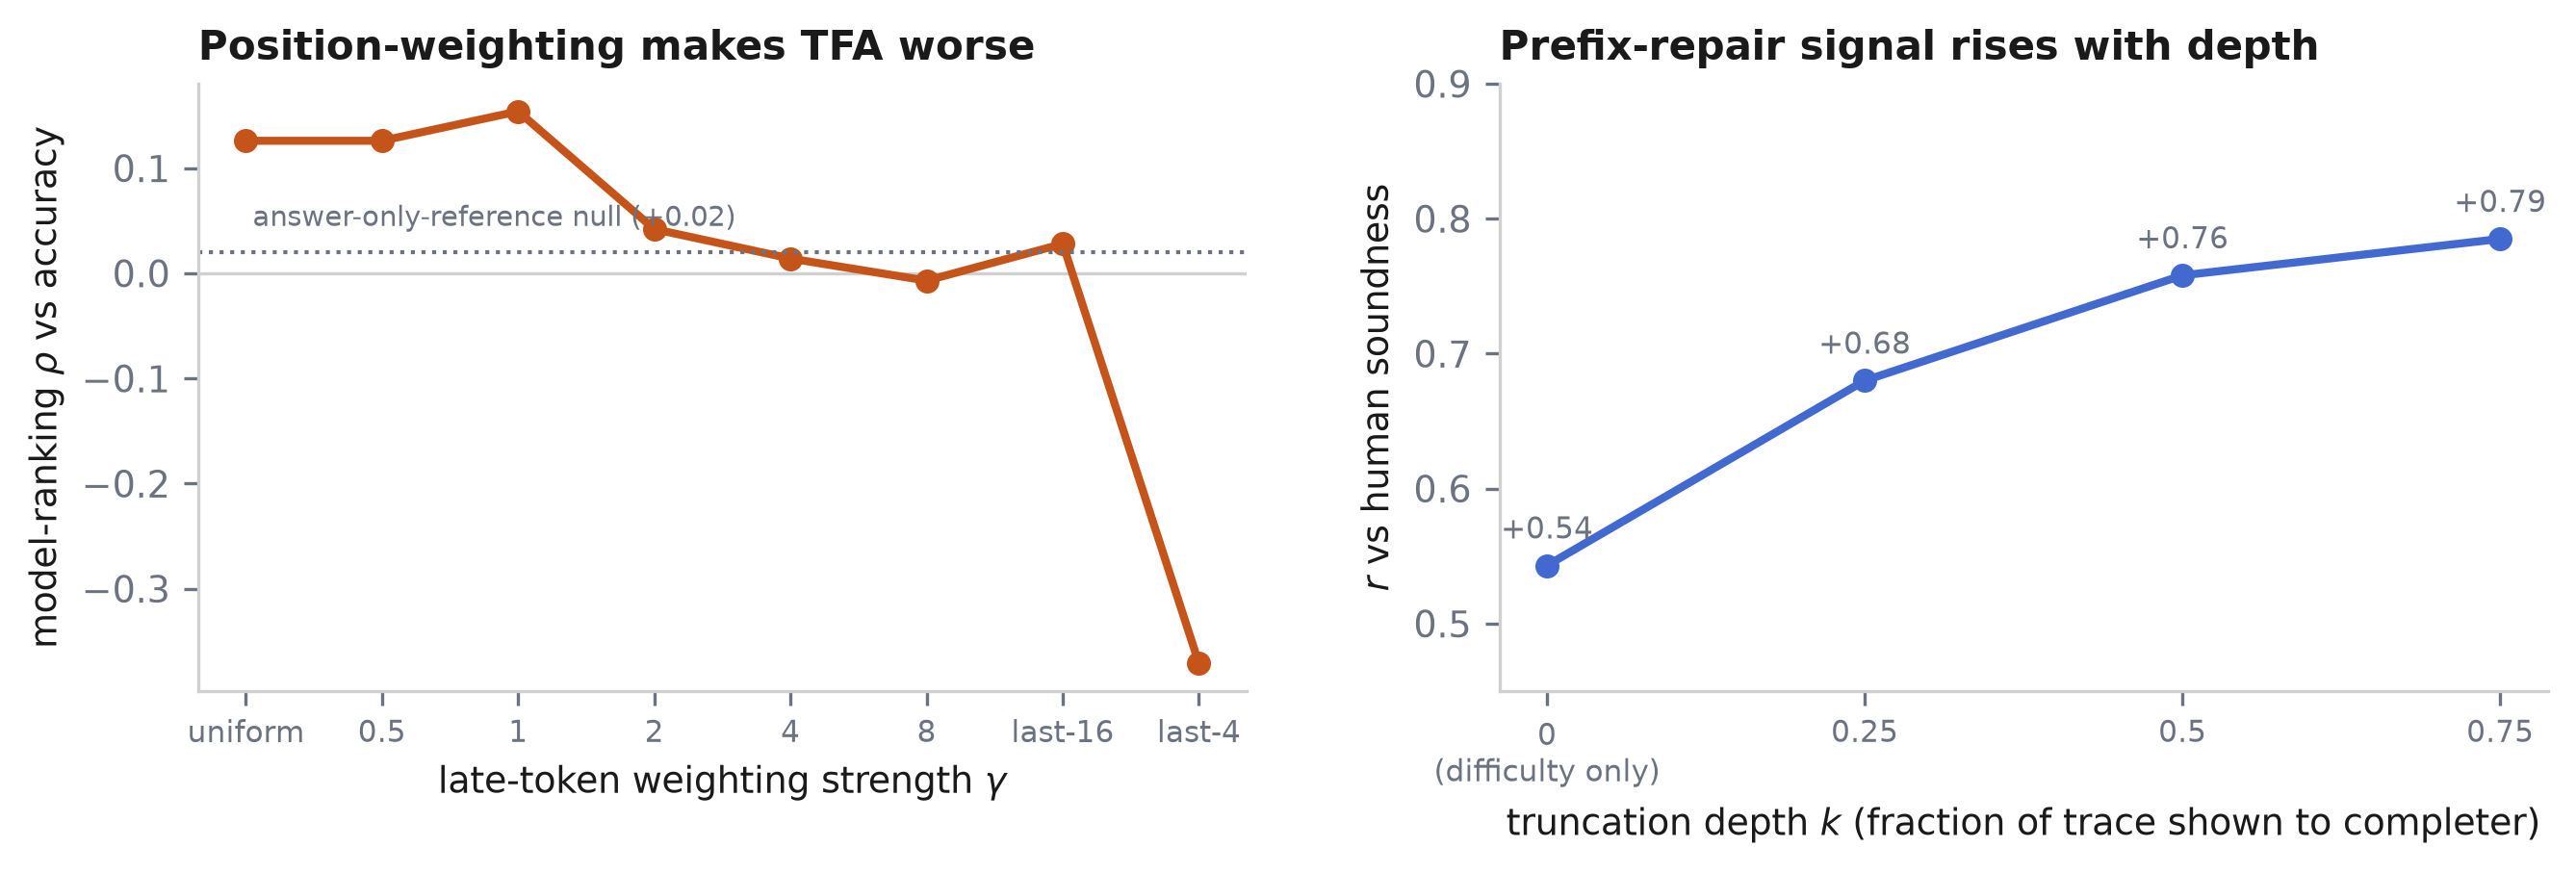
\includegraphics[width=0.9\textwidth]{figs/fig2_sweeps.png}
\caption{\textbf{The two registered sweeps move in opposite directions, as the taxonomy predicts.}
Left: up-weighting late reference tokens (the intuitive repair) decays \tfa's twelve-model ranking signal monotonically past $\gamma{=}1$, through the answer-only-reference null and beyond it.
Right: the prefix-repair signal rises monotonically with truncation depth, from a pure difficulty probe ($k{=}0$) to $+0.78$ against human soundness at $k{=}0.75$, with a curve mean of $+0.79$.}
\label{fig:sweeps}
\end{figure}

\section{What does grade: verification signals}
\label{sec:verify}

\emph{Executed tests} are the ceiling case: a free, perfect oracle wherever they exist, and the standard against which \tfa{} scored $0.00$.

\emph{The prefix-repair curve} is the strongest cheap signal we found.
Against the 60-item random label set, its correlation with soundness rises monotonically with truncation depth: $+0.54$ at $k{=}0$ (solving from scratch, a pure difficulty probe), $+0.68$ at $k{=}0.25$, $+0.76$ at $k{=}0.5$, and $+0.78$ at $k{=}0.75$ (Figure~\ref{fig:sweeps}, right).
The mean over the curve reaches $+0.79$ $[+0.61, +0.92]$.
This is the profile that ``the trace's reasoning causally supports its answer'' should produce.
Controlling for difficulty via the $k{=}0$ arm, the prefix's added completability still carries $+0.69$.
For scale: on the same labels every comparison metric sits at $|r| \le 0.33$, and the LLM judge reads \judgetbd.
The curve mean's $+0.79$ sits numerically at the human inter-rater reliability ceiling ($\rho = 0.79$, measured on the shared block), which is as high as any signal can be credited on these labels.
Its costs are real: about a hundred completions per solution, and a completer whose strength must sit in a middle band.
Too weak, and it cannot finish sound work; too strong, and it rescues broken work.

\emph{The answer-swap counterfactual} is the cheap end of the same class: one forward pass, no judge, no completion.
It is positive in 8 of 9 models (mean within-model $r = +0.13$, best $+0.34$), confirming the class prediction in direction while remaining too weak to use alone.
The ordering within the verification class (tests, then the repair curve, then answer-swap) tracks how much verification each performs, which is the taxonomy's internal consistency check.

Notice what the working signals have in common, and what they lack.
None treats the reference text as a target.
Executed tests consume the reference behavior, the prefix-repair curve uses only the reference's final answer as a checkable endpoint, and the answer-swap margin uses that answer as a counterfactual contrast.
Any metric that instead scores resemblance to the reference text inherits the nuisance decomposition of Section~\ref{sec:mechanism}, which is why the taxonomy could call the outcome of every entry in Table~\ref{tab:slate} in advance.
Where LLM judges fall in this taxonomy depends on their protocol; measuring that is the subject of companion work.

\section{Practical guidance}
\label{sec:rules}

\begin{enumerate}
\item \textbf{Never use a reference as a similarity target.}
Its value is as context for a reader or as a checkable endpoint for a verifier (Section~\ref{sec:verify}).
Any metric that scores resemblance to reference text inherits the nuisance decomposition of Section~\ref{sec:mechanism}, and the taxonomy correctly predicted the failure of every such metric before it was built.
In particular, matching scores should never be used as per-solution rewards or filters: the per-solution signal is not weak, it is absent, across the entire metric class, in two domains, against both human grades and executed tests.
\item \textbf{For leaderboards, matching is legitimate exactly when references are worth predicting.}
Report reference entropy alongside accuracy.
On answer-line references, matching measures style.
\end{enumerate}

\section{Limitations}
\label{sec:limits}

The human anchor is the 60-item random label set, graded by one annotator who is also an author, with a shared block graded by two annotators supplying the reliability ceiling.
A second rater on thirty random items and an external non-author annotator are pending, and the prefix-repair headline ($+0.79$) should be treated as provisional until they land.
The prefix-repair completer shares a model family with a subset of the graded traces, and its signal is substantially correctness-mediated: among correct-only solutions the $k{=}0.75$ point drops to $+0.19$ and the curve mean to $+0.07$.
All anchor-set numbers come from a single canonical analysis script (\texttt{papers/analysis/canonical\_validity.py}); earlier drafts and decks quoted values from heterogeneous scripts and estimators, and where they differ the canonical values supersede them.
Human-grade validity claims cover one math dataset plus executable code; a second labeled dataset is future work.
Pooled seventeen-model rankings have wide intervals, so we rest the ranking claims on the within-family ladders, which are individually consistent.

\section{Related work}
\label{sec:related}

Reliability audits of LLM judges conclude that reliability without validity is the field's open problem, and they call for variance-component analysis of the kind performed here~\cite{zheng2023judging,tan2024judgebench}.
Cheap reference-based metrics descend from text-generation evaluation~\cite{yuan2021bartscore}, where they are typically validated against human preferences of fluency; we test them against blind soundness grades and an executable oracle, and locate their variance in the reference itself.
The style-over-substance literature documents evaluator biases in general response pools~\cite{wu2023style,dubois2024length,singhal2023long}; our contribution is complementary, a mechanism (the reference-nuisance decomposition) and an intervention (the short-reference collapse) for reference-anchored metrics specifically.
Completion-based process values descend from rollout estimation in process supervision~\cite{lightman2023verify,wang2022selfconsistency}.
The prefix-repair curve, its monotone depth profile, and its difficulty-controlled reading appear to be new, as does the class-level advance-prediction test of the comparison/verification taxonomy.

\section{Conclusion}
\label{sec:conclusion}

Reference-based evaluation has been treated as a spectrum of increasingly good approximations to judgment.
It is not a spectrum.
It is two mechanisms.
Signals that compare a solution to reference text measure the reference: $80\%$ perplexity, $83$--$92\%$ item nuisance.
No reweighting recovers a grading signal, because there is none to recover.
Signals that verify a checkable endpoint grade in proportion to how much verification they perform, from a one-pass answer-swap margin, through the prefix-repair curve, to executed tests.
The boundary for leaderboard use is equally mechanistic: matching ranks models exactly when references are worth predicting, and reference entropy can be measured in advance to check that condition.
The taxonomy called the outcome of every new metric we built before the data existed, which is the strongest evidence that the divide is a mechanism and not a coincidence of this model grid.

\vspace{1em}
\noindent\textbf{Reproducibility.}
All scores, labels, decompositions, and pre-registered analysis scripts are in the repository (\texttt{experiments/tfa-vs-judge}): the class table (\texttt{runs/metric\_class\_results.md}), the decomposition (\texttt{scripts/two\_way\_decomp.py}), the short-reference intervention (\texttt{scripts/tfa\_shortref.py}), the metric slate (\texttt{scripts/analyze\_metric\_ablations.py}, \texttt{scripts/analyze\_slate2.py}), the executable oracle (\texttt{scripts/run\_code\_tests.py}), and the labeling instruments with returned labels (\texttt{human\_eval/}).

\appendix

\section{The full metric-class table}
\label{app:classtable}

All five comparison metrics under the same four tests: model-level boundary (hard-benchmark / \textsc{GSM8K} pooled $\rho$), variance decomposition (item / item$\times$family / residual shares, four families), and correlation with blind human soundness (the 60-item random label set).

\begin{table}[h]
\centering
\footnotesize
\setlength{\tabcolsep}{2.2pt}
\begin{tabular}{llccc}
\toprule
metric & mechanism & boundary (hard / sat.) & item / fam / resid \% & vs.\ human \\
\midrule
\tfa{} (argmax) & prediction fit & $+0.60$ / $-0.25$ & $83$--$92$ / $3$--$7$ / $5$--$11$ & $-0.16$ $[-0.46, +0.13]$ \\
gold-token logprob & prediction fit & $+0.43$ / $-0.23$ & $83$--$91$ / $7$--$11$ / $1$--$6$ & $-0.27$ $[-0.54, +0.04]$ \\
TF-IDF cosine & weighted similarity & $+0.72$ / $+0.12$ & $69$ / $8$ / $23$ & $-0.08$ $[-0.33, +0.18]$ \\
sentence embeddings & semantic similarity & $+0.87$ / $+0.29$ & $\sim$$70$ / $8$ / $21$ & $+0.14$ $[-0.08, +0.40]$ \\
unigram-F1 & raw overlap & $-0.49$ / $+0.18$ & $45$--$55$ / $12$--$15$ / $32$--$41$ & $-0.33$ $[-0.58, -0.12]$ \\
\midrule
LLM judge (referenced) & verification & --- & --- & \judgetbd{} $[+0.76, +0.97]$ \\
completion value ($k{=}0.5$) & verification & --- & --- & $+0.76$ $[+0.56, +0.91]$ \\
\bottomrule
\end{tabular}
\caption{Prediction-fit and weighted-similarity metrics rank on hard benchmarks and die or invert on saturated ones; raw overlap does not rank at all (its hard-benchmark inversion is a verbosity confound: controlling output length moves $-0.49$ to $-0.07$).
No comparison metric grades against human soundness; both verification signals do.
Human columns are Pearson $r$ with bootstrap 95\% CIs on the 60-item set; gold-token logprob uses the $n{=}42$ subset with logprob available.}
\label{tab:classfull}
\end{table}

\begin{thebibliography}{12}
\small
\bibitem{zheng2023judging} L.~Zheng et al. Judging LLM-as-a-Judge with MT-Bench and Chatbot Arena. arXiv:2306.05685, 2023.
\bibitem{tan2024judgebench} S.~Tan et al. JudgeBench: A Benchmark for Evaluating LLM-Based Judges. arXiv:2410.12784, 2024.
\bibitem{wu2023style} M.~Wu and A.~F.~Aji. Style Over Substance: Evaluation Biases for Large Language Models. arXiv:2307.03025, 2023.
\bibitem{dubois2024length} Y.~Dubois et al. Length-Controlled AlpacaEval: A Simple Way to Debias Automatic Evaluators. arXiv:2404.04475, 2024.
\bibitem{singhal2023long} P.~Singhal et al. A Long Way to Go: Investigating Length Correlations in RLHF. arXiv:2310.03716, 2023.
\bibitem{lightman2023verify} H.~Lightman et al. Let's Verify Step by Step. arXiv:2305.20050, 2023.
\bibitem{wang2022selfconsistency} X.~Wang et al. Self-Consistency Improves Chain of Thought Reasoning in Language Models. arXiv:2203.11171, 2022.
\bibitem{yuan2021bartscore} W.~Yuan, G.~Neubig, and P.~Liu. BARTScore: Evaluating Generated Text as Text Generation. arXiv:2106.11520, 2021.
\bibitem{hendrycks2021math} D.~Hendrycks et al. Measuring Mathematical Problem Solving With the MATH Dataset. arXiv:2103.03874, 2021.
\bibitem{cobbe2021gsm8k} K.~Cobbe et al. Training Verifiers to Solve Math Word Problems. arXiv:2110.14168, 2021.
\bibitem{chen2021codex} M.~Chen et al. Evaluating Large Language Models Trained on Code. arXiv:2107.03374, 2021.
\bibitem{austin2021mbpp} J.~Austin et al. Program Synthesis with Large Language Models. arXiv:2108.07732, 2021.
\bibitem{liu2023evalplus} J.~Liu et al. Is Your Code Generated by ChatGPT Really Correct? Rigorous Evaluation of Large Language Models for Code Generation. arXiv:2305.01210, 2023.
\end{thebibliography}

\end{document}
